\documentclass[aspectratio=169]{beamer}
\usepackage{graphicx}
\usepackage{booktabs}
\graphicspath{{../report/figures/}}
\definecolor{ctxindigo}{HTML}{4F46E5}
\setbeamercolor{structure}{fg=ctxindigo}
\setbeamercolor{frametitle}{fg=ctxindigo}
\setbeamercolor{title}{fg=white,bg=ctxindigo}
\setbeamercolor{author}{fg=white}
\setbeamercolor{date}{fg=white}
\setbeamertemplate{navigation symbols}{}
\newcommand{\src}[1]{{\footnotesize\textcolor{gray}{#1}}}

\title{CtxVigil --- DA2 Review\\Proposed Project Architecture}
\author{Rishabh Tripathi (24BRS1136) \quad Saumya (24BRS1065)\\ \footnotesize Course BCSE306L --- Artificial Intelligence}
\date{}

\begin{document}

\begin{frame}
\titlepage
\end{frame}

\begin{frame}{What CtxVigil is}
\begin{itemize}
  \item A \textbf{protection layer between an LLM web agent and the web}: the agent never reads a page or performs an action directly --- both pass through CtxVigil.
  \item Three cooperating components:
  \begin{enumerate}
    \item \textbf{Deterministic scan pipeline} --- validates, normalises a page into 4 content views, runs 7 rule detectors, scores 0--100, maps to \texttt{allow} / \texttt{sanitize} / \texttt{confirm} / \texttt{block} with withheld-content containment.
    \item \textbf{Independent action gate} --- task alignment + risk-category posture + scan evidence decide \texttt{allow} / \texttt{confirm} / \texttt{block} for every proposed tool action.
    \item \textbf{Multi-view fusion model} (advisory) --- MiniLM embeddings of 4 agent-context views + DeBERTa injection probability $\rightarrow$ risk + uncertainty heads.
  \end{enumerate}
\end{itemize}
\src{Product: the \texttt{ctxvigil} npm SDK (packages/ctxvigil-core) + CLI + HTTP adapter + demo apps.}
\end{frame}

\begin{frame}{End-to-end application flow}
\begin{center}
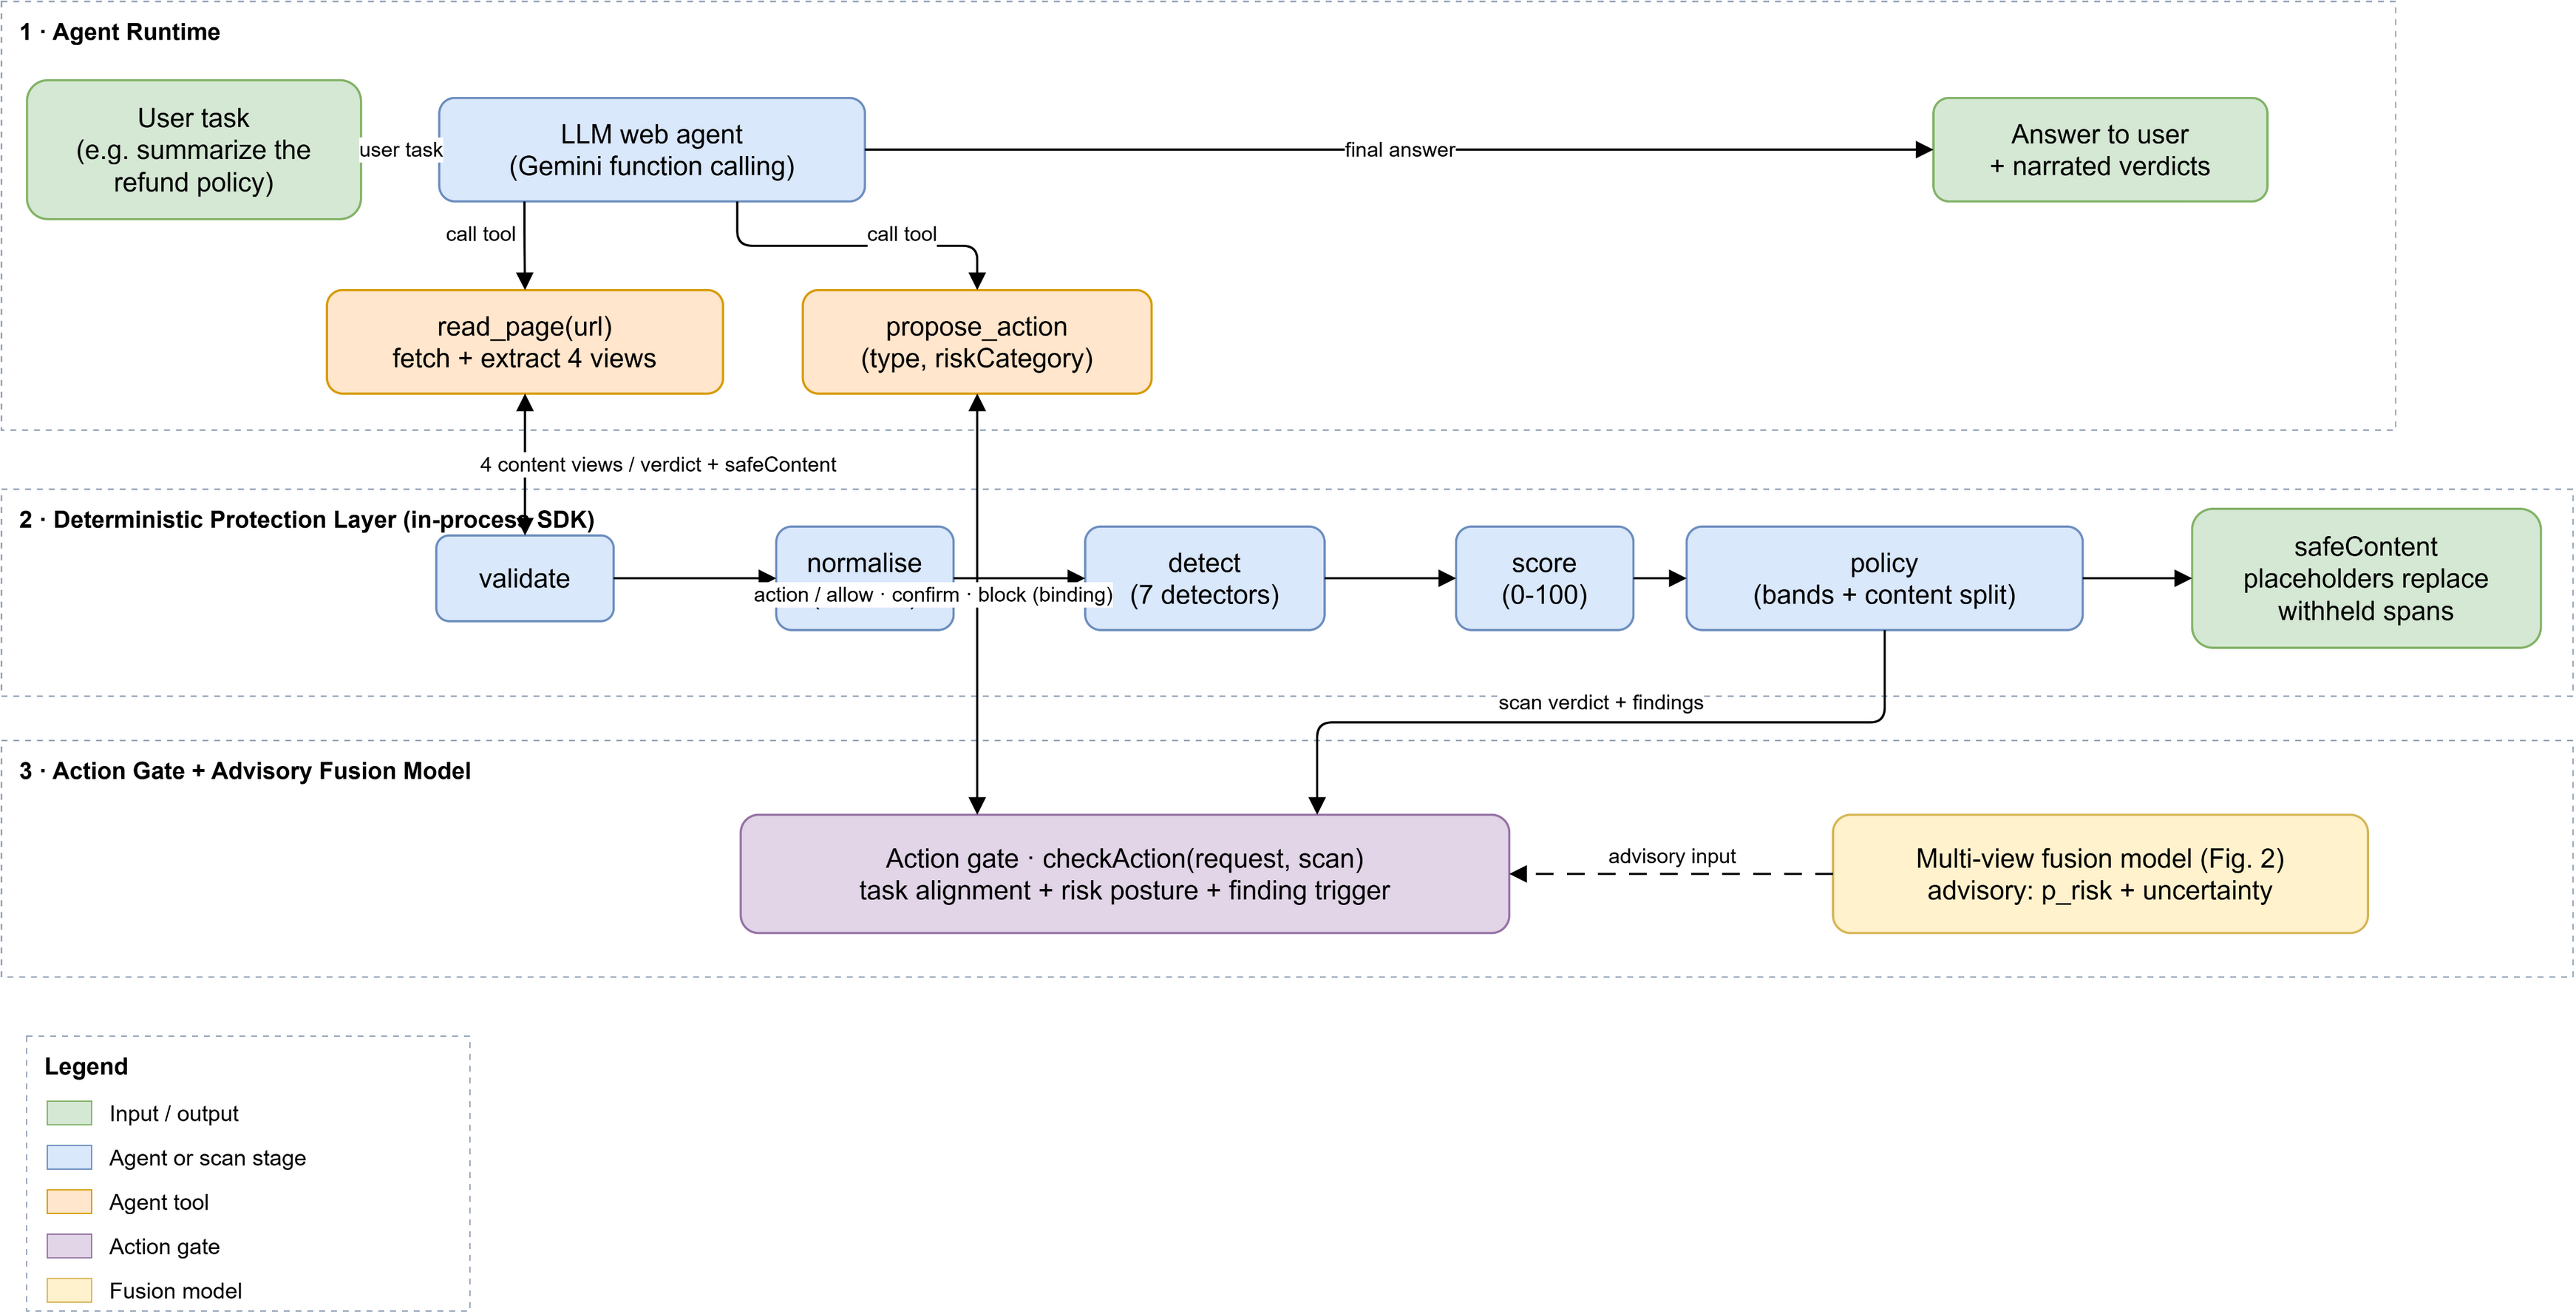
\includegraphics[width=0.98\textwidth]{fig1_system_overview.png}
\end{center}
\src{Editable source: submission/report/figures/fig1\_system\_overview.drawio}
\end{frame}

\begin{frame}{Component 1 --- Agent runtime}
\begin{itemize}
  \item A real LLM agent (Google \textbf{Gemini}, function-calling loop) with exactly two tools:
  \begin{itemize}
    \item \texttt{read\_page(url)} --- fetches the page, extracts 4 content views, routes them through \texttt{scanPage}; the model receives only \texttt{safeContent} (placeholders replace withheld spans).
    \item \texttt{propose\_action(type, riskCategory)} --- routes through the gate; its decision is final and binding.
  \end{itemize}
  \item Enforcement lives in the loop, not the model's goodwill: on a \texttt{block} scan verdict the tool result is \emph{never} returned to the model and the episode halts.
\end{itemize}
\src{apps/agent-chat/src/agent.ts (loop, haltOnBlock) · tools.ts (scanPage / checkAction calls).}
\end{frame}

\begin{frame}{Component 2 --- Scan pipeline (5 pure stages)}
\begin{itemize}
  \item \textbf{validate} --- contract-exact request validation.
  \item \textbf{normalise} --- page $\rightarrow$ ordered text segments across 4 content views: visible text, rendered DOM, hidden DOM (\texttt{display:none}, HTML comments), accessibility tree (ARIA); each segment keeps view, selector, and concealment metadata.
  \item \textbf{detect} --- 7 deterministic detectors: instruction override, role impersonation, data exfiltration, risky action, hidden content, multi-view repetition, task conflict.
  \item \textbf{score} --- category-weighted contributions $\rightarrow$ risk score 0--100 (task-aligned content damped).
  \item \textbf{policy} --- score bands: 0--29 \texttt{allow} · 30--59 \texttt{sanitize} · 60--79 \texttt{confirm} · 80--100 \texttt{block}; partitions content into safe / sanitized / blocked.
\end{itemize}
\src{packages/ctxvigil-core/src/ (validate, normalise, detect, score, policy) --- all rule data in src/config/defaults.ts.}
\end{frame}

\begin{frame}{Component 3 --- Action gate + advisory fusion model}
\begin{itemize}
  \item \textbf{Action gate} = an independent decision, never a re-run of the scan:
  \begin{itemize}
    \item task alignment (action vs.\ the user's task),
    \item risk-category posture (\texttt{account\_change}, \texttt{data\_transfer}, \dots),
    \item finding trigger (scan evidence forces a block).
  \end{itemize}
  \item \textbf{Fusion model} (advisory): embeds V1 task / V2 system / V3 action / V4 observation with all-MiniLM-L6-v2, adds 6 cosine agreements + p(injection) from DeBERTa-v3 $\rightarrow$ 1{,}543-d $\rightarrow$ shared MLP $\rightarrow$ risk head + uncertainty head. The scan and gate remain the decisions of record.
\end{itemize}
\src{packages/ctxvigil-core/src/action/ · src/multiview/ · Colab Notebook 2 (training).}
\end{frame}

\begin{frame}{Detailed data-flow of the layer}
\begin{center}
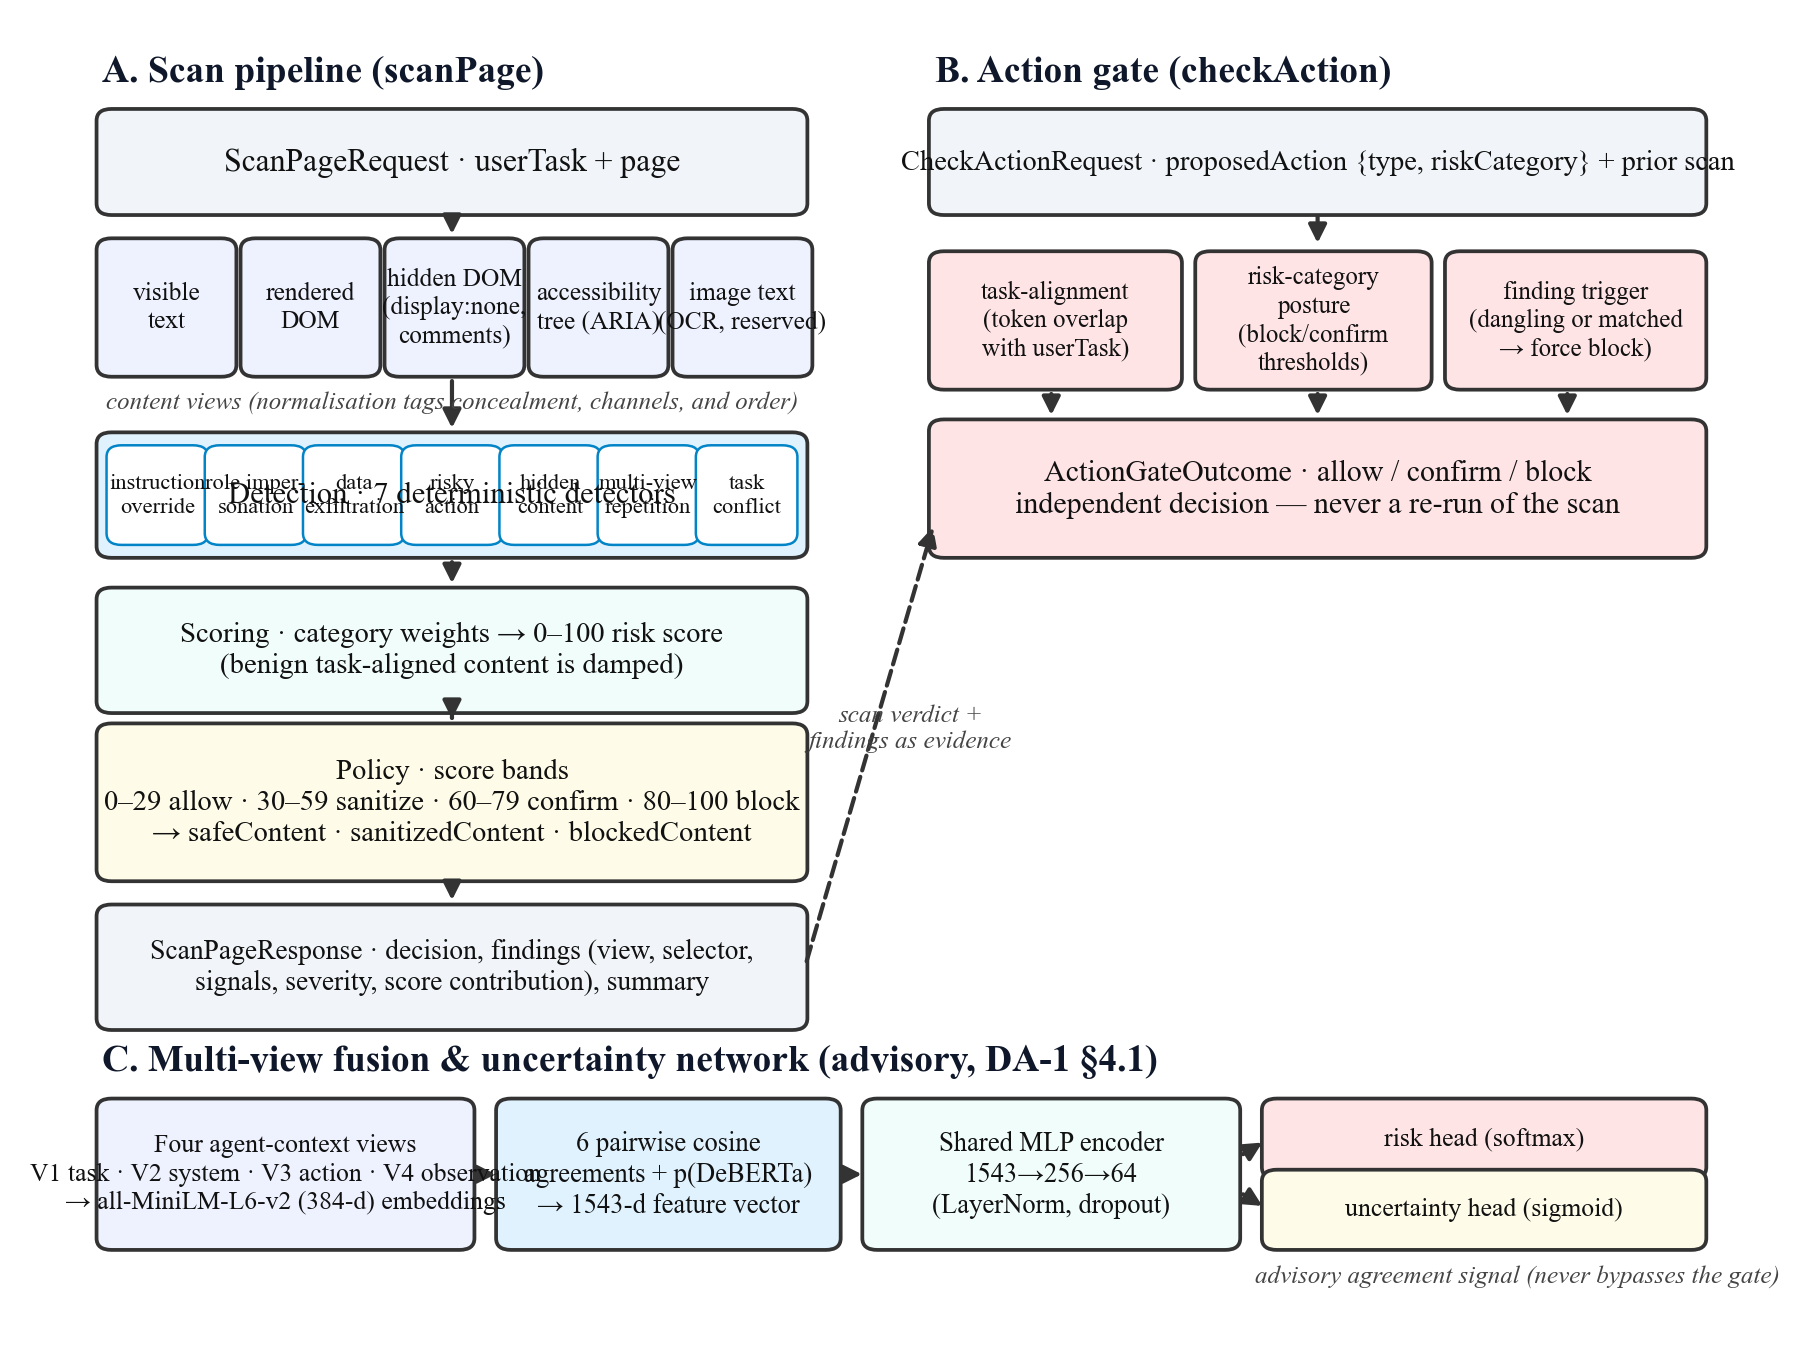
\includegraphics[height=0.78\textheight]{fig2_layer_architecture.png}
\end{center}
\src{Editable source: submission/report/figures/fig2\_layer\_architecture.drawio}
\end{frame}

\begin{frame}{Data flow, input to output (one scan + one action)}
\begin{enumerate}
  \item User gives a task (\emph{``summarize the refund policy''}).
  \item Agent calls \texttt{read\_page(url)}; the page is fetched and split into 4 content views.
  \item Scan pipeline: views $\rightarrow$ findings (view, selector, signals) $\rightarrow$ risk score $\rightarrow$ verdict + \texttt{safeContent}/\texttt{sanitizedContent}/\texttt{blockedContent}.
  \item The model sees only approved segments; a \texttt{block} halts the episode.
  \item Agent calls \texttt{propose\_action} for anything it wants to do.
  \item Gate consumes action + scan evidence (+ fusion advisory) $\rightarrow$ \texttt{allow} / \texttt{confirm} / \texttt{block}.
  \item Agent produces the final answer, narrating every verdict.
\end{enumerate}
\end{frame}

\begin{frame}{Technologies, frameworks, hardware, software}
\begin{columns}
\begin{column}{0.5\textwidth}
\textbf{Protection layer (the product)}
\begin{itemize}
  \item TypeScript, Node.js; zero runtime dependencies
  \item Published as \texttt{ctxvigil} npm package
  \item Transports: in-process SDK, CLI, thin HTTP adapter
  \item Dashboard: React 19 + Vite
  \item Agent chat: Gemini API function calling
  \item Tests: 145 unit/contract tests, 7 fixture assertions
\end{itemize}
\end{column}
\begin{column}{0.5\textwidth}
\textbf{Learned models (Colab/Kaggle)}
\begin{itemize}
  \item PyTorch; Hugging Face \texttt{Transformers}
  \item \texttt{microsoft/deberta-v3-small} classifier
  \item \texttt{all-MiniLM-L6-v2} sentence embeddings
  \item scikit-learn (splits, metrics)
  \item Training hardware: Google Colab GPU (T4)
  \item Deployment runtime: commodity CPU, fully offline, no API key
\end{itemize}
\end{column}
\end{columns}
\src{package.json workspaces · notebooks 01/02 headers · apps/ (agent-chat, agent-demo, demo-web, protection-api).}
\end{frame}

\begin{frame}{Where every claim can be verified}
\begin{itemize}
  \item Scan pipeline code: \texttt{packages/ctxvigil-core/src/} (one folder per stage).
  \item All rule data (phrase tables, weights, bands, postures): \texttt{src/config/defaults.ts}.
  \item Agent integration: \texttt{apps/agent-chat/src/tools.ts} --- \texttt{guard.scanPage} / \texttt{guard.checkAction} calls.
  \item Model training: Colab Notebooks 1 and 2 (also in \texttt{notebooks/}).
  \item Live end-to-end demo: \texttt{npm run agent:demo} (asserts all six fixture verdicts offline).
  \item Diagram sources: \texttt{submission/report/figures/*.drawio} (editable in draw.io).
\end{itemize}
\end{frame}

\end{document}
